\chapter{Generación del documento de texto}

En este Capítulo se diseñará e implementará el proceso de generación del Documento de Texto, teniendo en mente los procesos conocidos de la GLN vistos anteriormente. Usaremos el Árbol de Entidades del Organizador de Información detallado en el Capítulo~\ref{cap:organizacion} para dar una estructura inicial al texto, y luego verbalizaremos los Constructores de la Ontología, teniendo en cuenta la coherencia local dentro de los párrafos generados.

\section{Introducción}
Para abordar el proceso de generación de texto, se tomó como referencia las actividades de la Generación de Lenguaje Natural nombradas en la Sección~\ref{sec:tareas_gnl}. Se crearon tres módulos principales: Macroplanificador, Microplanificador y Realizador, los cuales implementan los procesos asociados a las etapas de Macroplanificación, Microplanificación y Realización gramatical, respectivamente. Dentro de cada módulo se desarrollaron submódulos, para resolver cada problema específico. 

Elegimos organizar toda la información de la ontología generando un documento dividido en secciones, subsecciones y párrafos. 

Como presentamos en el Objetivo (Sección~\ref{Intro:objetivo}), se esperan alcanzar dos cualidades principales en el texto de salida:
\begin{enumerate}
    \item A nivel macro: el texto debe tener una estructura que permita visualizar los principales temas, presentándolos de manera aislada (secciones, párrafos), pero que en conjunto se complementen para que el lector pueda establecer las relaciones adecuadas entre ellos. Como objetivo principal se espera alcanzar una estructura que presente la información más importante y necesaria lo más temprana posible, preparando al lector para que pueda comprender información nueva.
    \item A nivel micro, el texto debe cumplir con cierta fluidez, utilizando frases que tengan una gramática aceptable, tratando de maximizar la cohesión.
\end{enumerate}

Para satisfacer las necesidades del nivel macro, usaremos como punto de partida la estructura resultante del módulo de Organización de Información, que servirá para generar un Documento Inicial. Este Documento Inicial se modificará para adoptar una estética más agradable para el lector, tratando de mantener la coherencia global de la estructura original.

Parte de la estética resulta de crear secciones y párrafos con los tópicos del texto. Dado que queremos dotar al texto con coherencia local, debemos definir qué información habrá en cada sección y párrafo, y cómo estará organizada. 

Tomando algunos postulados básicos de la Teoría de Centrado, contamos con una base inicial para elegir cómo presentar en lenguaje natural y de manera coherente la información contenida en la ontología. No es el objetivo de este trabajo implementar una solución basada estrictamente en las reglas propuestas por dicha Teoría, más bien, se pretende alcanzar una cierta coherencia local motivados por la idea que subyace en la misma.

Para mantener la coherencia local según la Teoría de Centrado, debemos evitar cambiar continuamente los focos de atención. Por este motivo, para cada tópico tratado en el texto, trataremos de capturar y presentar toda su información agrupada en párrafos consecutivos.  

Dado una entidad \emph{E}, para recuperar la información que la describe, adoptaremos dos criterios principales:
\begin{itemize}
    \item El primer criterio consiste en juntar los axiomas que describen a \emph{E} en un mismo párrafo. %Los axiomas de cada entidad están guardados en la estructura de la ontología creada en el módulo \emph{Traductor} del capítulo anterior, por lo que obtenerlos y agruparlos es trivial.
    \item El segundo criterio consiste en recorrer la estructura de grafo a partir del nodo que representa a \emph{E}, navegando por las relaciones del nodo. Este recorrido busca capturar la máxima cantidad de información posible acerca de \emph{E}. 
\end{itemize}

Estos criterios permiten desarrollar el texto tomando centralmente a cada entidad una sola vez, de manera que el foco de atención solo salte hacia otras entidades cuando no haya nada más para decir acerca de \emph{E}.


En el nivel micro, debemos definir una traducción desde la gramática del lenguaje OWL 2 hacia el lenguaje humano. Luego se modificará convenientemente la traducción para alcanzar el Documento Final, generando un texto más fluido y organizando las sentencias para maximizar la cohesión.

La relación entre el Organizador de Información y el Generador del Documento de Texto se puede ver en la Figura~\ref{fig:modulos_sgln}.

\begin{figure}
    \centering
    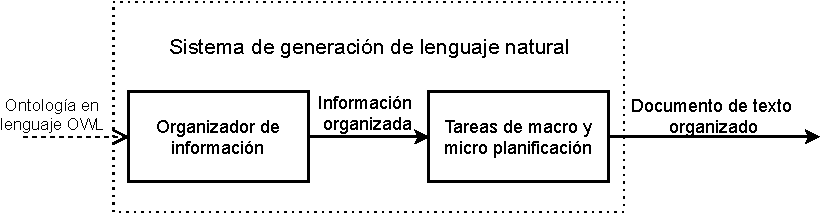
\includegraphics{img/presentacion_problema/modulos_sgln.pdf}
    \caption{Módulos que componen el Sistema de Generación de Lenguaje Natural}
    \label{fig:modulos_sgln}
\end{figure}


Ampliando el módulo \emph{Generador de Documento de Texto} en la Figura~\ref{fig:modulos_documento_final}, se puede apreciar el flujo de información entre los módulos desarrollados en este Capítulo.

\begin{figure}
    \centering
    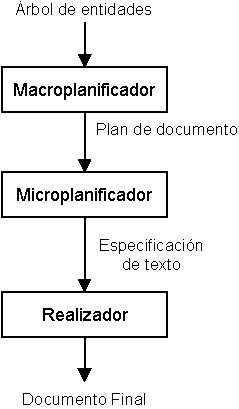
\includegraphics{img/generacion_documento/modulos_documento_final.pdf}
    \caption{Módulos para la generación del Documento Final.}
    \label{fig:modulos_documento_final}
\end{figure}


\section{Diseño Macroplanificador}
\label{sec:macro_planning}
En esta etapa se planificará la estructura del documento. Como nombramos anteriormente, la organización a priori de la información, realizada en el capítulo anterior, facilita la tarea de Macroplanificación. Para crear el documento en la etapa de Macroplanificación, se reemplazó el módulo Generador del Árbol de Entidades del Organizador de Información, por un nuevo módulo específico del Macroplanificador. El motivo de este reemplazo es evitar la creación de interfaces entre el Organizador de Información y el Macroplanificador, por el \emph{overhead} que estas suponen, ya que la creación del Árbol de Entidades y la Macroplanificación resultan ser procesos equivalentes, por lo que pueden ser reemplazables, evitando recorrer el doble de veces la estructura jerárquica.

En la Figura~\ref{fig:modulos_plan_documento} se puede ver el nuevo módulo Generador del Plan de Documento, que retorna como salida un Plan de Documento.

\begin{figure}
    \centering
    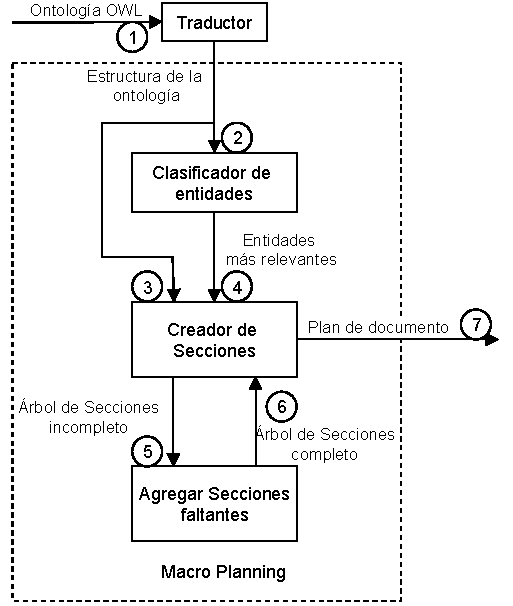
\includegraphics{img/generacion_documento/modulos_plan_documento.pdf}
    \caption{Módulos para la generación del Plan de Documento.}
    \label{fig:modulos_plan_documento}
\end{figure}

El documento de texto estará representado internamente con una estructura basada en componentes. Esta representación prepara el terreno para que, luego de la Microplanificación, el Realizador decida el diseño final del documento.

La representación interna del documento de texto tiene en cuenta los siguientes criterios:
\begin{itemize}
    \item Cada\textit{ Entidad} presente en la estructura que resulta del Organizador de Información es considerada un tópico. 
    \item A cada\textit{ Tópico} del primer nivel le corresponde una sección. Los tópicos anidados (Subclases, Individuos y Relaciones) se corresponden a subsecciones (secciones anidadas).
    \item Cada \textit{Sección} está compuesta de al menos un párrafo y un título.
    \item Cada \textit{Párrafo} trata un único tópico, el cual puede ser una clase o un individuo. También, un párrafo puede o no tener alguna sentencia. Esto se debe a que no todas las entidades tienen asociados axiomas que la describan.
\end{itemize}

\subsection{Secciones y párrafos}
Las Secciones tiene como objetivo principal delimitar la información asociada a una Entidad, segmentando el texto con el fin de mantener la coherencia global.

Dentro de una sección para una Clase, se verbalizarán sus axiomas y se enumerarán sus Individuos, Subclases y Relaciones, todo en un párrafo. Enumerar esta información (es decir, presentarla sin considerarla un nuevo tópico) resulta conveniente ya que luego se crearán subsecciones para cada uno de esos componentes.

En una sección asociada a una Relación, solo habrán subsecciones acerca de las Entidades que pertenecen a la Relación.

En una sección para Individuos, se creará un párrafo para describir sus propiedades.

\subsubsection{Subsecciones}
Las subsecciones son secciones anidadas dentro de otras secciones. Una subsección puede surgir a partir de un Individuo, Subclases o Relaciones. Cuando surge a partir de un Individuo, la subsección trata como tópico al Individuo; cuando surge a partir de una Subclase, el tópico principal es la Subclase; y cuando surge a partir de una Relación, el tópico principal resulta ser el rango de la Relación, es decir, otra Clase.

\subsection{Oraciones}
Las oraciones pertenecen a los párrafos por lo que tratan un solo tópico. Cada oración que tenga como tópico a una Clase,  aborda un solo tipo de información, por lo que existe una oración para las clases disjuntas, una oración para las clases equivalentes, y así con los demás tipos de información. Cada oración correspondientes a un Individuo contiene las propiedades con sus valores declaradas sobre el Individuo.

Al tratar un solo tipo de información por oración, se maximiza la cohesión dentro de cada oración.


\subsection{Diagrama de clases}
En la Figura~\ref{fig:diagrama_clases_macroplanificador} se muestra el diagrama de clases correspondiente al Macroplanificador. La clase \emph{TextManager} es la implementación del módulo Generador del Plan de Documento. Esta clase se encarga de crear la clase \emph{Text}, que es la representación interna de un documento de texto. El documento está compuesto por Secciones, Párrafos y Oraciones, cada uno de los cuales tiene asociado su respectiva clase \emph{Section}, \emph{Paragraph} y \emph{Statement}.

\begin{figure}
    \centering
    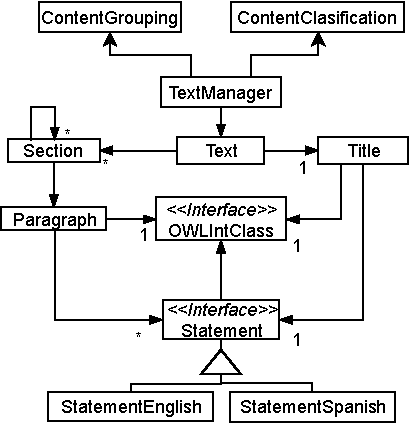
\includegraphics{img/generacion_documento/diagrama_clases_macroplanificador.pdf}
    \caption{Diagrama de clases del Macroplanificador.}
    \label{fig:diagrama_clases_macroplanificador}
\end{figure}

\section{Implementación Macroplanificador}
La clase principal del Macroplanificador es \emph{TextManager}. Para crear el Documento Inicial, recorre las Entidades de la misma manera que la clase \emph{GeneratorTreeManager}, explicada en la Figura~\ref{sec:clase_generator_tree}, con la diferencia que crea el objeto \emph{Text} y los objetos \emph{Section} asociados a cada Entidad. Ya que el recorrido es equivalente no se presentará su implementación, en cambio comenzaremos a mostrar las clases que componen el Documento de Texto.

La clase \emph{Text} solo contiene los objetos del primer nivel del Documento de Texto. Tiene acceso a las secciones principales y a las secciones que contienen la información que no había sido utilizada en otras secciones. 

La clase \emph{Section} contiene la información referida a una Sección, como título, párrafos, sus subsecciones y el tópico asociado. Implementa el método de realización del Documento Final, el cual se verá en el Capítulo de Realización.

Cada \emph{Section} se encarga de crear el \emph{Paragraph} correspondiente a su Tópico.

La clase \emph{Paragraph} contiene una lista de todas las \emph{Statement} referidas a su Tópico. 

Cada \emph{Paragraph} se encarga de crear las \emph{Statement} correspondientes para el Tópico que recibe, y asociarles los componentes (Axiomas) que describen al Tópico. Adicionalmente el párrafo recibe el lenguaje del texto, por lo que debe instanciar las \emph{Statement} adecuadas, ya sea \emph{StatementEnglish} o \emph{StatementSpanish}.

La clase \emph{Statement} contiene la información que tendrá cada oración. Será usada por el Microplanificador para verbalizar la información e implementar los métodos de la etapa de Microplanificación. 

\section{Diseño Microplanificador}
En esta estapa se llevarán a cabo las tareas para describir una Entidad en lenguaje natural a partir de la información que contiene cada \emph{Statement} creada en la Macroplanificación. Esta descripción en lenguaje natural se alcanza a través de una o varias oraciones producidas con una estructura que se adapte a la gramática del lenguaje español.

Como existen diversas estructuras sintácticas para expresar un mismo contenido, a modo de simplificación se asoció a cada constructor OWL solo algunas formas de verbalización. Se trató de generar oraciones que sean fieles al significado expresado en los axiomas y de evitar ambigüedades.

Para poder trabajar con patrones de la gramática del lenguaje humano (ya sea español o inglés), se utilizó un \emph{POS Tagger}\footnote{Un \emph{Part-Of-Speech Tagger} es un software para asignar la categoría gramatical a las palabras de un texto.} para etiquetar las palabras. Se eligió usar \emph{Stanford POS Tagger}\footnote{https://nlp.stanford.edu/software/tagger.html}, el cual tiene una API en lenguaje Java para integrar fácilmente al proyecto. Siendo un software basado en modelos probabilísticos, \emph{Stanford POS Tagger} posee una alta efectividad (sobre 97\% para el inglés), y una rápida velocidad de ejecución.

\subsection{Verbalización de una oración}
Tanto las oraciones acerca de Clases como las de Individuos requieren la verbalización de los constructores OWL. Solo en el caso de las oraciones acerca de Clases requieren además la enumeración de sus instancias, propiedades y subclases. Con enumeración de las propiedades (y de instancias y subclases por igual), nos referimos únicamente a presentarlas, por ejemplo, las propiedades \emph{tieneCobertura} y \emph{tieneBase} para la clase Pizza resultan en la oración ``una pizza tiene base de pizza y tiene cobertura de pizza''.

Las tareas necesarias para la verbalización de una oración son:
\begin{itemize}
    \item Verbalizar los constructores OWL o enumerar las propiedades, instancias y subclases.
    \item Eliminar información redundante entre oraciones a través del proceso de agragación.
    \item En el caso de las Clases, se reemplaza con expresiones de referencia a los nombres de las Clases en oraciones consecutivas evitando que se repitan y que genere un texto poco fluido.
\end{itemize}

\subsection{Sintaxis OWL 2}
\label{sec:gen_doc_sintaxis_owl}
Teniendo en cuenta la estructura jerárquica de la sintaxis (a partir de su gramática BNF y de los diagramas de clases de su documentación~\cite{OWL2W3C}), agrupamos en diferentes niveles de abstracción las tres categorías sintácticas: en el nivel inferior se encuentran las Entidades, en el nivel intermedio las Expresiones de Clases, y en el nivel superior los Axiomas. Esta separación en niveles de abstracción será útil para organizar la verbalización. El conjunto de constructores elegido para verbalizar se encuentra en las siguientes listas: en la lista~\ref{list:constructores_axiomas} se agrupan los constructores del nivel de Axiomas, en la Lista~\ref{list:constructores_expresiones} los constructores de Expresiones de Clases y en la lista~\ref{list:constructores_entity} los constructores de nivel de Entidades.
\begin{figure}
\begin{multicols}{2}
\captionof{listCap}{Constructores de Entidades}
\label{list:constructores_entity}
    \begin{itemize}
        \item owl:class
        \item owl:objectProperty
        \item owl:dataProperty
        \item owl:individual
        \item[\vspace{\fill}]
    \end{itemize}

\captionof{listCap}{Constructores de Axiomas}
\label{list:constructores_axiomas}
    \begin{itemize}
        \item rdfs:subClassOf
        \item owl:equivalentClass
        \item owl:disjointWith
        \item rdfs:domain
        \item rdfs:range
    \end{itemize}
    \end{multicols}
\end{figure}


\begin{figure}
\captionof{listCap}{Constructores de Expresiones de Clase}
\label{list:constructores_expresiones}
    \begin{itemize}
    \begin{multicols}{2}
        \item owl:intersectionOf
        \item owl:unionOf
        \item owl:complementOf
        \item owl:allValuesFrom
        \item owl:someValuesFrom 
        \item owl:minCardinality
        \item owl:maxCardinality
        \item owl:Cardinality
        \item owl:oneOf
        \item owl:hasValue
        \end{multicols}
    \end{itemize}
\end{figure}

\subsection{De OWL 2 a lenguaje natural}
La verbalización de la sintaxis OWL 2 se corresponde a la tarea de traducir el lenguaje OWL al lenguaje humano. Para llevar a cabo la traducción, se tendrán en cuenta los niveles de abstracción presente en la Sección~\ref{sec:gen_doc_sintaxis_owl}. 

El enfoque adoptado para crear la sintaxis de las oraciones se basa en un recorrido bottom-up de la jerarquía de un \textit{Axioma}. Se comienza desde las hojas, construyendo oraciones parciales a partir de las\textit{ Entidades}, luego se procede a subir por los niveles a través de los constructores de\textit{ Expresiones de Clases}, componiendo nuevas oraciones parciales, hasta alcanzar la raíz de la jerarquía, donde se termina de construir la oración final. Adicionalmente, se realizan algunos tratamientos morfológicos para agregar fluidez y coherencia al texto, tal como insertar artículos, y hacer concordar los sustantivos en género y número.

Con el objetivo de comenzar a formar las oraciones parciales, el primer paso a realizar es la verbalización de las \textit{Entidades}, ya que están directamente relacionadas con las IRIs (o tienen acceso al \emph{label}, en caso de extraer los nombres desde los \emph{labels}).

En la Gramática~\ref{gram:entity} se muestra una porción de la gramática BNF del lenguaje OWL 2 asociada a las Entidades.
\begin{GrammarEnv}
%detecta un error de sintaxis pero es mentira.
\begin{grammar}
[(colon){$\rightarrow$}]
[(semicolon)$|$]
[(comma){}]
[(period){\vspace{0.3cm} \\}]
[(quote){\begin{bf}}{\end{bf}}]
[(nonterminal){$<$}{$>$}]
%<expression> : <number> ; <number>, [\{"asd"\}], <relational\_operator>, <number>.
%<number> : <digit> ; <digit> , <number>.
%<digit> : "0";"1";"2";"3";"4";"5";"6";"7";"8";"9".
%<relational\_operator> : $"="$;"$\lessthan \greaterthan$";"$\lessthan$";"$\greaterthan$"; "$\lessthan=$";"$\greaterthan=$";"in".
\fbox{\begin{minipage}{14cm} \small{ 
<Entity> : <Class> ; <ObjectProperty> ; <DataProperty> ; <NamedIndividual> ; <AnnotationProperty>.
<Class> : <IRI> .
<ObjectProperty> : <IRI> .
<DataProperty> : <IRI> .
<AnnotationProperty> : <IRI> .
<NamedIndividual> : <IRI> .
}
\end{minipage}
}
\end{grammar}
\caption{Porción de gramática asociada a las Entidades.}\label{gram:entity}
\end{GrammarEnv}

En el siguiente nivel se tienen los constructores de \textit{Expresiones de Clase}, con las cuales es posible generar oraciones complejas subordinando las expresiones que se encuentran anidadas, o componer nuevas oraciones parciales teniendo en cuenta los tipos de componentes involucrados.

En la Gramática~\ref{gram:expr_clases} se muestra a modo de ejemplo una sección de la gramática con constructores de este nivel.
\begin{GrammarEnv}
\begin{grammar}
[(colon){$\rightarrow$}]
[(semicolon)$|$]
[(comma){}]
[(period){\vspace{0.3cm} \\}]
[(quote){\begin{bf}}{\end{bf}}]
[(nonterminal){$<$}{$>$}]
%<expression> : <number> ; <number>, [\{"asd"\}], <relational\_operator>, <number>.
%<number> : <digit> ; <digit> , <number>.
%<digit> : "0";"1";"2";"3";"4";"5";"6";"7";"8";"9".
%<relational\_operator> : $"="$;"$\lessthan \greaterthan$";"$\lessthan$";"$\greaterthan$"; "$\lessthan=$";"$\greaterthan=$";"in".
\fbox{\begin{minipage}{14cm} \small{ 
<ClassExpression> : <Class> ; <ObjectIntersectionOf> ; <ObjectSomeValuesFrom> .
<ObjectSomeValuesFrom> : "ObjectSomeValuesFrom" "(" <ObjectPropertyExpression> <ClassExpression> ")" .
<ObjectPropertyExpression> : <ObjectProperty> .
}
\end{minipage}}
\end{grammar}
\caption{Porción de gramática asociada a las Expresiones de Clases.}\label{gram:expr_clases}
\end{GrammarEnv}

Puede apreciarse en la gramática que existe recursividad entre los constructores, lo que produce que un constructor aparezca en diferentes niveles y pueda combinarse con cualquier otro constructor del nivel de \textit{Expresiones de Clases.} En este punto es importante que cada constructor pueda componerse con los demás, para asegurar cualquier combinación posible.

Por último en el nivel más abstracto se encuentran los constructores de \textit{Axiomas}. Estos constructores tienen la característica de no ser recursivos entre ellos, por lo que es posible generar oraciones independientes, yuxtapuestas o coordinadas. Un ejemplo de estos constructores se ve en la Gramática~\ref{gram:axiom}.

\begin{GrammarEnv}
\begin{grammar}
[(colon){$\rightarrow$}]
[(semicolon)$|$]
[(comma){}]
[(period){\vspace{0.3cm} \\}]
[(quote){\begin{bf}}{\end{bf}}]
[(nonterminal){$<$}{$>$}]
%<expression> : <number> ; <number>, [\{"asd"\}], <relational\_operator>, <number>.
%<number> : <digit> ; <digit> , <number>.
%<digit> : "0";"1";"2";"3";"4";"5";"6";"7";"8";"9".
%<relational\_operator> : $"="$;"$\lessthan \greaterthan$";"$\lessthan$";"$\greaterthan$"; "$\lessthan=$";"$\greaterthan=$";"in".
\fbox{\begin{minipage}{14cm} \small{ 
<ClassAxiom> : <SubClassOf> ; <EquivalentClasses> ; <DisjointClasses> ; <DisjointUnion> .
<EquivalentClasses> : "EquivalentClasses" "(" <axiomAnnotations> <ClassExpression> <ClassExpression> \{ <ClassExpression> \} ")".
}
\end{minipage}}
\end{grammar}
\caption{Porción de gramática asociada a los Axiomas.}\label{gram:axiom}
\end{GrammarEnv}

\subsection{Componentes y oraciones parciales}
Durante la creación de una oración, se recorren los constructores de\textit{ Expresiones de Clases} y de \textit{Entidades}, creando oraciones parciales y componiéndolas entre ellas. Dado que cada constructor puede componerse con cualquier otro y en cualquier nivel de profundidad, se decidió asociar a cada constructor un tipo de componente oracional, de esta manera se evita una exhaustiva programación de composiciones.
Los tipos de componentes son los siguientes:
\begin{itemize}
    \item Término (T): caracterizado por no poseer verbo. Pueden contener adverbios, sustantivos y adjetivos.
    \item Sintagma Verbal (SV): debe poseer un verbo.
    \item Oración Negativa (ON): representa la negación de un componente.
    \item Unión: representa una disyunción de oraciones parciales.
    \item Intersección: representa una adición o subordinación de oraciones parciales.
\end{itemize}

Estos tipos de componentes definen un sistema de tipos, en el que cada tipo puede componerse con otro y dan como resultado un nuevo componente. El tipo de una composición depende del constructor que opere con esos componentes.
%En la mayoría de los casos el tipo de componente es predecible, a excepción de la \emph{intersección}.

Los componentes que retorna cada constructor se definen a continuación:
\begin{itemize}
    \item Componente Término (T):
    \begin{itemize}
        \item Clase.
        \item Individuo
    \end{itemize}
    \item Componente Sintagma Verbal (SV):
    \begin{itemize}
        \item Propiedad.
        \item Constructores de cuantificación.
        \item Constructor \emph{hasValue}.
        \item Constructores con cardinalidad.
    \end{itemize}
    \item Componente Union: 
    \begin{itemize}
        \item \emph{UnionOf}.
        \item \emph{OneOf}
    \end{itemize}
    
    \item Componente Intersección: solo el constructor \emph{IntersectionOf}.
    \item Componente Oración Negativa (ON): solo el constructor \emph{ComplementOf}.
\end{itemize}

El beneficio de este sistema es que cada constructor sabe cómo realizar la composición, en función del tipo de cada uno de sus operandos, lo que reduce la cantidad de combinaciones a programar (en contraste con tener que programar el proceso de composición de cada constructor teniendo en cuenta que sus operandos serían otros constructores en lugar de componentes). 

Además, incorporar un sistema como este, evita el uso de otras técnicas menos afines a la lingüística, como \emph{templates} prediseñados o texto genérico para cada caso particular, ya que se basa en el uso de patrones más cercanos a la Lingüística Teórica, apoyando el uso de teorías lingüísticas en el campo del Procesamiento de Lenguaje Natural.


Sin embargo, estos componentes no intentan ser exhaustivos ni completamente fieles a la sintaxis del lenguaje humano, sino que intentan acaparar de la forma más general los posibles resultados de cada constructor, para mantener una sintaxis sencilla y aceptable. Una \textit{Clase}, por ejemplo, podría cumplir la función de sintagma nominal, adjetival o adverbial, pero para simplificar la nomenclatura, se retorna un tipo más genérico y al momento de usar una \textit{Clase}, de ser necesario, se resuelve la composición en función de los elementos que la constituyen. Como veremos más adelante, a veces es innecesario discriminar los tipos de sintagmas.


\subsection{Convención y suposiciones del nombrado de Entidades}
Para no limitar la aplicación a una convención de nombrado, no se requiere una forma estricta para nombrar las entidades en una ontología. Sin embargo, nos basamos en algunas suposiciones que resultan natural al crear una ontología:
\begin{enumerate}
    \item Las entidades pueden tener su nombre ya sea en la IRI o en un label\footnote{Estas opciones son excluyentes, al verbalizar una ontología solo se extraen los nombres de un solo lugar, por lo que todos los nombres deben ser extraídos de IRI o de label sin combinarse}. Si el nombre es extraído de una IRI, debe estar escrito con el estilo CamelCase. Si el nombre se extrae de un label, debe estar escrito en lenguaje natural, y debe tener el idioma del label (en este caso, español ``es'' o ingles ``en'').
    \item No hay condiciones para el nombre de una clase, sin embargo es preferible que contenga al menos un sustantivo.
    \item No hay condiciones para el nombre de una propiedad, sin embargo es preferible que contenga al menos un verbo. 
    
    No es conveniente omitir las preposiciones finales, por ejemplo, en la propiedad \emph{esParte}, es recomendable utilizar \emph{esParteDe}. Por otro lado, si el nombre contiene un verbo, no se infieren los mismos, por lo que si se quiere expresar, por ejemplo, que una clase \emph{está localizada en} algún lugar, la propiedad debería llamarse \emph{estáLocalizadaEn} y no \emph{localizadaEn}. 
    
    % No se infieren verbos, por lo que si se quiere expresar, por ejemplo, que una clase \emph{está localizada en} algún lugar, la propiedad debería llamarse \emph{estáLocalizadaEn} y no \emph{localizadaEn}. Al igual que los verbos, no es conveniente omitir las preposiciones finales, por ejemplo, enla propiedadesParte, es recomendable utilizaresParteDe
\end{enumerate}

Estas condiciones ayudan a mejorar la fluidez del texto y no suponen una gran carga en los desarrolladores de ontologías.
%Sin embargo, se considerado como trabajo futuro de esta investigación.

De hecho, existen varios trabajos que abordan la nomenclatura de conceptos, especificando convenciones de nombrado para el desarrollo de las ontologías, coincidiendo en algunos aspectos (y siendo hasta más estrictos) con nuestros requerimientos~\cite{montiel2011style}~\cite{OntoCheck}.

\subsection{Tratamiento sintáctico de los nombres de Entidades}
Para facilitar el entendimiento de las secciones referidas a la Microplanificación, se explicará cómo fueron tratados los nombres de las entidades, desde el punto de vista sintáctico. 

Dado que los nombres de las\textit{ Entidades} pueden no corresponderse fielmente con la gramática de un lenguaje (por falta de palabras funcionales, tales como artículos o preposiciones), se optó por no realizar un análisis sintáctico a los nombres. Sin embargo, para soportar la creación de patrones gramaticales, se etiquetaron las palabras de cada \textit{Entidad }para reconocer la función gramatical de cada una y poder llevar a cabo las composiciones.

Se consideró, a cada conjunto de palabras que conforman el nombre de una entidad, como un componente incompleto (oración parcial) que es parte de una oración más grande. Por este motivo, se divide en dos partes fundamentales: una parte inicial y un complemento, entre los cuales pueden insertarse nexos y cuantificaciones. A continuación se explican cómo se reconocen ambas partes en las clases y propiedades:
\begin{itemize}
    \item Los nombres de las propiedades (en los que suponemos existe al menos un verbo), se considera como parte inicial a todas las palabras desde el inicio hasta el primer verbo, incluído el verbo. El complemento se conforma con todas las palabras que siguen al verbo. Por ejemplo: la propiedad \emph{tiene color} se compone de parte inicial: \emph{tiene}, y complemento: \emph{color}. La propiedad \emph{se solapa con} se compone de \emph{se solapa} como parte de inicial, y \emph{con} como complemento.
    \item Para las clases (en las que suponemos existe al menos un sustantivo), se considera como parte inicial a todas las palabras desde el inicio hasta el primer sustantivo, incluido el sustantivo. El complemento se conforma con todas las palabras que siguen al sustantivo. Por ejemplo: la clase \emph{agente social}, tiene como parte inicial \emph{agente} y complemento \emph{social}. La clase \emph{cobertura de pizza} se compone de \emph{cobertura} con complemento \emph{de pizza}.
    \item Los nombres de los individuos son tratados igual que los nombres de las clases.
\end{itemize}


\subsection{Verbalización de constructores OWL}
\label{sec:verbalizacion_constructores}
Esta tarea se encarga de componer las oraciones según la información de cada constructor OWL.
%Las oraciones pueden enfocarse ya sea en una \emph{owl:Class} o  \emph{owl:NamedIndividual}. Cuando se enfocan en una \emph{owl:Class}, pueden contener la siguiente información: clases equivalentes, disjuntas y superclases. Cuando se enfoca en un \emph{owl:NamedIndividual}, puede contener información acerca de los valores de sus propiedades.
%Para cada uno de estos tipos de información, se pueden presentar una o varias oraciones. Las oraciones que tratan el mismo tipo de información se organizan adyacentemente entre ellas.
En algunos constructores, tener un único patrón gramatical resulta insuficiente, debido a que pueden recibir distintas estructuras gramaticales como entrada, que requieren diferentes formas de componerse. Por lo tanto, en estos casos se diseñó más de una forma de composición, mejorando la variabilidad, fluidez e interpretación de las oraciones. 

Para reconocer cómo componer las oraciones en cada constructor, se revisó empíricamente los axiomas de algunas ontologías, y se buscó utilizar oraciones que sean lo más genéricas posibles, que permitan la comprensión de los axiomas. 

A continuación se explican los patrones gramaticales usados para cada constructor. %El signo $+$ corresponde a la concatenación de cadenas de texto.

\subsubsection{Restricción de cardinalidad \emph{ObjectCardinalityRestriction}}

La Gramática~\ref{gram:object_card_rest} muestra los patrones diseñados para las restricciones de cardinalidad sobre \emph{objectProperty}. En los casos donde sea posible, si la clase sobre la que se aplica la restricción es \emph{owl:Thing}, se reemplaza por el rango de la propiedad, el complemento de la propiedad (como el {\tt patron$_2$}) o por último por la palabra ``cosa''.

El enlace es seleccionado dependiendo del operador \emph{MinCardinality}, \emph{MaxCardinality} y \emph{ExactCardinality}.

Ejemplo: para la clase ``pizza interesante'', se tiene el axioma: ``tieneCobertura min 3 owl:Thing''. Dado que la restricción se aplica sobre la clase \emph{owl:Thing}, en la verbalización se busca reemplazar esa clase por una oración que sea más significativa. Existen dos posibilidades, una es utilizar el complemento de la propiedad (elaborado en el patron$_2$), y la otra es utilizar el rango de la propiedad \emph{tieneCobertura} (elaborado en el patron$_3$). Como en este caso la propiedad tiene definido su rango, resulta más informativo utilizar el rango, que utilizar el complemento de la propiedad. Si se eligiera el patron$_2$, se obtendría la oración ``tiene \texttt{como mínimo} 3 coberturas'', mientras que utilizar el patron$_3$ genera la oración ``tiene \texttt{como mínimo} 3 coberturas de pizza''. Las gramáticas siempre buscan utilizar oraciones con la mayor información posible, evitando oraciones genéricas como ``tiene \texttt{como mínimo} 3 cosas'', por eso en este caso se elige usar el patron$_3$.

\begin{GrammarEnv}
\begin{grammar}
[(colon){$\rightarrow$}]
[(semicolon)$|$]
[(comma){}]
[(period){\vspace{0.3cm} \\}]
[(quote){\begin{bf}}{\end{bf}}]
[(nonterminal){$<$}{$>$}]
\fbox{\begin{minipage}{14cm} \small{ 
<RestriccionCard> : <patron$_1$> ; <patron$_2$> ; <patron$_3$> ; <patron$_4$> .
<patron$_1$> : <parteInicialPropiedad> <complementoPropiedad> <enlace> <cardinalidad> <clases> .
<patron$_2$> : <parteInicialPropiedad> <enlace> <cardinalidad> <complementoPropiedad>.
<patron$_3$> : <parteInicialPropiedad> <enlace> <cardinalidad> <rangoPropiedad>.
<patron$_4$> : <parteInicialPropiedad> <enlace> <cardinalidad> <clases>.
<enlace> : "como mínimo" ; "como máximo"; "exactamente".
}
\end{minipage}}
\end{grammar}
\caption{Patrones para ObjectCardinalityRestriction.}\label{gram:object_card_rest}
\end{GrammarEnv}

\subsubsection{Restricción de cardinalidad \emph{DataCardinalityRestriction}}
La Gramática~\ref{gram:data_card_rest} muestra los patrones diseñados para las restricciones de cardinalidad sobre \emph{dataProperty}. El {\tt patron$_2$} es específico para cuando la propiedad no tiene verbo. 

\begin{GrammarEnv}
\begin{grammar}
[(colon){$\rightarrow$}]
[(semicolon)$|$]
[(comma){}]
[(period){\vspace{0.3cm} \\}]
[(quote){\begin{bf}}{\end{bf}}]
[(nonterminal){$<$}{$>$}]
\fbox{\begin{minipage}{14cm} \small{ 
<RestriccionCard> : <patron$_1$> ; <patron$_2$>.
<patron$_1$> : <parteInicialPropiedad> <enlace> <cardinalidad> <complementoPropiedad> .
<patron$_2$> : "tiene" <enlace> <cardinalidad> <nombrePropiedad>.
<enlace> : "al menos" ; "como máximo"; "exactamente".
}
\end{minipage}}
\end{grammar}
\caption{Patrones para DataCardinalityRestriction.}\label{gram:data_card_rest}
\end{GrammarEnv}

\subsubsection{Restricción de cuantificación \emph{QuantifiedObjectRestriction}}
La Gramática~\ref{gram:quant_obj_rest} muestra los patrones diseñados para las cuantificaciones sobre \emph{objectProperty}.

\begin{GrammarEnv}
\begin{grammar}
[(colon){$\rightarrow$}]
[(semicolon)$|$]
[(comma){}]
[(period){\vspace{0.3cm} \\}]
[(quote){\begin{bf}}{\end{bf}}]
[(nonterminal){$<$}{$>$}]
\fbox{\begin{minipage}{14cm} \small{ 
<RestriccionQuant> : <patron$_1$> ; <patron$_2$> ; <patron$_3$> ; <patron$_4$> ; <patron$_5$> .
<patron$_1$> : <parteInicialPropiedad> "como" <complementoPropiedad> <enlace> <clases> .
<patron$_2$> : <parteInicialPropiedad> <enlace> <complementoPropiedad> "$\colon$" <clases> .
<patron$_3$> : <parteInicialPropiedad> <enlace> "a" <clases> .
<patron$_4$> : <parteInicialPropiedad> "a" <enlace> <clases> .
<patron$_5$> : <parteInicialPropiedad> <complementoPropiedad> <enlace> <clases> .
<enlace> : "algún" ; "alguna"; "algo"; "exclusivamente" .
}
\end{minipage}}
\end{grammar}
\caption{Patrones para QuantifiedObjectRestriction.}\label{gram:quant_obj_rest}
\end{GrammarEnv}

Los enlaces dependen del tipo de cuantificador y del tipo de palabra que lo proceda. Si el cuantificador es existencial, el enlace sería ``alguna/algún'' para palabras que sean sustantivo femenino o masculino respectivamente, o con cualquier otra palabra sería ``algo''.  Para el cuantificador universal el enlace es siempre ``exclusivamente''. Adicionalmente, si posee una enumeración de clases (es decir que $<$clases$>$ posee más de una clase), se agrega al enlace la conexión ``las/los siguientes''.

Ejemplo: la clase ``Margherita'' que es subclase de ``PizzaConNombre'', tiene el axioma ``tieneCobertura only 
    (CoberturaDeMozzarella or CoberturaDeTomate)'' (siendo only el cuantificador universal), el cual se traduce con el patron$_2$ a ``tiene \texttt{exclusivamente las siguientes} coberturas: cobertura de mozzarella o cobertura de tomate''. También posee dos axiomas equivalentes al anterior: ``tieneCobertura some CoberturaDeMozzarella'' y ``tieneCobertura some CoberturaDeTomate'', (siendo some el cuantificador existencial), los cuales se traducen con patron$_1$ a ``tiene \texttt{como} cobertura \texttt{a alguna} cobertura de mozzarella'' y ``tiene \texttt{como} cobertura \texttt{a alguna} cobertura de tomate''.


\subsubsection{Restricción de cuantificación \emph{QuantifiedDataRestriction}}
La Gramática~\ref{gram:quant_data_rest} muestra los patrones diseñados para las cuantificaciones sobre \emph{dataProperty}.

\begin{GrammarEnv}
\begin{grammar}
[(colon){$\rightarrow$}]
[(semicolon)$|$]
[(comma){}]
[(period){\vspace{0.3cm} \\}]
[(quote){\begin{bf}}{\end{bf}}]
[(nonterminal){$<$}{$>$}]
\fbox{\begin{minipage}{14cm} \small{ 
<RestriccionQuant> : <patron$_1$> ; <patron$_2$> .
<patron$_1$> : <verboPropiedad> <enlace> <complementoPropiedad> "de tipo" <rangoPropiedad> .
<patron$_2$> : <verboPropiedad> <complementoPropiedad> <enlace> "de tipo" <rangoPropiedad> .
<enlace> : "algún" ; "alguna"; "algo"; "exclusivamente" .
}
\end{minipage}}
\end{grammar}
\caption{Patrones para QuantifiedDataRestriction.}\label{gram:quant_data_rest}
\end{GrammarEnv}

\subsubsection{Restricción \emph{OWLObjectComplementOf}}
La Gramática~\ref{gram:complement_rest} muestra los patrones diseñados para el complemento de una Expresión de Clase.

\begin{GrammarEnv}
\begin{grammar}
[(colon){$\rightarrow$}]
[(semicolon)$|$]
[(comma){}]
[(period){\vspace{0.3cm} \\}]
[(quote){\begin{bf}}{\end{bf}}]
[(nonterminal){$<$}{$>$}]
\fbox{\begin{minipage}{14cm} \small{ 
<RestriccionComplement> : <patron$_1$>.
<patron$_1$> : <enlace> <clase> .
<enlace> : "lo opuesto de" ; "no"; "ni"; "excepto" .
}
\end{minipage}}
\end{grammar}
\caption{Patrones para OWLObjectComplementOf.}\label{gram:complement_rest}
\end{GrammarEnv}

El enlace depende del tipo de componente que retorne $<$clase$>$:
\begin{itemize}
    \item Si retorna T utiliza \texttt{lo opuesto de}.
    \item Si retorna SV utiliza \texttt{no}.
    \item Si retorna ON utiliza \texttt{ni}.
    \item En cualquier otro caso usa \texttt{excepto}.
\end{itemize}

\subsubsection{Restricción \emph{OWLObjectInverseOf}}
La Gramática~\ref{gram:inverse_rest} muestra los patrones diseñados para el inverso de una Propiedad.

\begin{GrammarEnv}
\begin{grammar}
[(colon){$\rightarrow$}]
[(semicolon)$|$]
[(comma){}]
[(period){\vspace{0.3cm} \\}]
[(quote){\begin{bf}}{\end{bf}}]
[(nonterminal){$<$}{$>$}]
\fbox{\begin{minipage}{14cm} \small{ 
<RestriccionInverse> : <patron$_1$>.
<patron$_1$> : <enlace> <Propiedad> .
<enlace> : "es lo opuesto de" .
}
\end{minipage}}
\end{grammar}
\caption{Patrones para OWLObjectInverseOf.}\label{gram:inverse_rest}
\end{GrammarEnv}

\subsubsection{Restricción \emph{OWLObjectHasValue}}
La Gramática~\ref{gram:hasvalue_rest} muestra los patrones diseñados para los valores de una Propiedad.

\begin{GrammarEnv}
\begin{grammar}
[(colon){$\rightarrow$}]
[(semicolon)$|$]
[(comma){}]
[(period){\vspace{0.3cm} \\}]
[(quote){\begin{bf}}{\end{bf}}]
[(nonterminal){$<$}{$>$}]
\fbox{\begin{minipage}{14cm} \small{ 
<RestriccionHasValue> : <patron$_1$> ; <patron$_2$>.
<patron$_1$> : <parteInicialPropiedad> <complementoPropiedad> <Individuo>.
<patron$_2$> : <parteInicialPropiedad> <Individuo> .
}
\end{minipage}}
\end{grammar}
\caption{Patrones para OWLHasValue.}\label{gram:hasvalue_rest}
\end{GrammarEnv}

\subsubsection{Restricción \emph{OWLObjectHasSelf}}
La Gramática~\ref{gram:hasself_rest} muestra los patrones diseñados para una auto restricción de una Propiedad sobre sí misma.

\begin{GrammarEnv}
\begin{grammar}
[(colon){$\rightarrow$}]
[(semicolon)$|$]
[(comma){}]
[(period){\vspace{0.3cm} \\}]
[(quote){\begin{bf}}{\end{bf}}]
[(nonterminal){$<$}{$>$}]
\fbox{\begin{minipage}{14cm} \small{ 
<RestriccionHasSelf> : <patron$_1$>.
<patron$_1$> : <parteInicialPropiedad> <complementoPropiedad> "Sí MISMO".
}
\end{minipage}}
\end{grammar}
\caption{Patrones para OWLObjectHasSelf.}\label{gram:hasself_rest}
\end{GrammarEnv}


\subsubsection{Restricción N-Ary \emph{UnionOf} y \emph{oneOf}} 
Como representan una secuencia de elementos, en la que uno o más elementos pueden ser verdaderos, se eligió concatenar a todos los elementos con el conector disyuntivo ``\textbf{o}''.  
Sean $e_1, e_2,\ldots,e_N$ los elementos de la enumeración, el patrón gramatical elegido es: $e_1, e_2,\ldots,e_{N-1}$ {\textbf{o}} $e_N$''.

\subsubsection{Restricción N-Ary \emph{InterseccionOf}}
La intersección da lugar tanto a la adición como a la subordinación de oraciones. Antes de verbalizar una intersección, se ordenan sus componentes de mayor a menor prioridad, teniendo en cuenta que: T, ON, Unión, Intersección tienen  igual prioridad, y SV contando con una menor prioridad que los anteriores componentes. 

Para determinar cómo verbalizar una intersección, se tienen en cuenta las siguientes condiciones:
\begin{itemize}
    \item Si la intersección tiene dos operandos:
        \begin{itemize}
            \item Si el primero es de tipo T  y el segundo SV, se subordina la segunda oración de la siguiente manera:
            ``contenido primer operando + \textbf{que} + contenido segundo operando''
            \item en cualquier otro caso, se coordinan los operandos:
            ``contenido primer operando + \textbf{y} + contenido segundo operando''
        \end{itemize}
        \item Si la intersección tiene más de dos operandos, se agrupan según el tipo  (T, SV, ON) y luego se coordinan con la conjunción ``y''.
\end{itemize}

Por ejemplo, el axioma de clase equivalente ``Pizza and (tieneCobertura some (CoberturaDePizza and (tienePicante some MuyPicante)))'' de la clase pizzaPicanteEquivalente, contiene dos intersecciones las cuales poseen los mismos componentes: T$+$SV, por lo que utilizamos el conector \textbf{que} para subordinar el segundo operando. Con este criterio, el axioma anterior sería ``pizza picante es una pizza \textbf{que} tiene alguna cobertura de pizza {\textbf{que}} tiene algún picante muy picante''.

En caso de asociar la intersección al conector \textbf{y} sin tener en cuenta el contexto, se generaría una oración como la siguiente ``pizza picante es una pizza \textbf{y} tiene alguna cobertura de pizza \textbf{y} tiene algo muy picante'', dando lugar a ambigüedad, pues la segunda \textbf{y} podría cumplir la función de adición, interpretándose que la pizza tiene algo picante, en lugar de cumplir una función de subordinación, donde la interpretación correcta es que la cobertura de la pizza es picante. 

\subsection{Enumeración de propiedades, subclases e individuos}
Enumerar esta información es solo para anunciar la existencia de estos componentes, por lo que la sintaxis es simple.

Para las subclases se crearon los patrones de la Gramática~\ref{gram:subclases}.
Para los individuos se crearon patrones similares al de las subclases.
Para las propiedades se crearon los patrones de la Gramática~\ref{gram:propiedades}.

\begin{GrammarEnv}
\begin{grammar}
[(colon){$\rightarrow$}]
[(semicolon)$|$]
[(comma){}]
[(period){\vspace{0.3cm} \\}]
[(quote){\begin{bf}}{\end{bf}}]
[(nonterminal){$<$}{$>$}]
\fbox{\begin{minipage}{14cm} \small{ 
<EnumerarSubclases> : <patron$_1$> ; <patron$_2$>.
<patron$_1$> : "existen las siguientes clases de" <topico> "$\colon$" <subclases>.
<patron$_2$> : <subclase> "es la única clase de" <topico>.
}
\end{minipage}}
\end{grammar}
\caption{Patrones para enumerar subclases.}\label{gram:subclases}
\end{GrammarEnv}

\begin{GrammarEnv}
\begin{grammar}
[(colon){$\rightarrow$}]
[(semicolon)$|$]
[(comma){}]
[(period){\vspace{0.3cm} \\}]
[(quote){\begin{bf}}{\end{bf}}]
[(nonterminal){$<$}{$>$}]
\fbox{\begin{minipage}{14cm} \small{ 
<EnumerarPropiedades> : <patron$_1$> ; <patron$_2$> ; <patron$_3$>.
<patron$_1$> : <parteInicialPropiedad> <complementoPropiedad> <rangoPropiedad> .
<patron$_2$> : <parteInicialPropiedad> "como" <complementoPropiedad> "a" <rangoPropiedad> .
<patron$_3$> : <parteInicialPropiedad> <rangoPropiedad> .
}
\end{minipage}}
\end{grammar}
\caption{Patrones para enumerar propiedades.}\label{gram:propiedades}
\end{GrammarEnv}



\subsection{Expresiones de referencia}
El proceso de referenciación se ve facilitado por el uso de la Teoría de Centrado. 
Teniendo en cuenta que cada párrafo (y por lo tanto cada oración que lo compone) trata centralmente una única \textit{Clase }o \textit{Individuo}, no se intercalan tópicos como focos de atención, por lo que se reduce la posibilidad de ambigüedad. Las expresiones de referencia solo fueron implementadas para las \textit{Clases}.

Para llevar a cabo la referenciación, se tuvo en cuenta el uso de pronombres demostrativos (``este/esta''), a veces, acompañados por el primer sustantivo (si posee) del nombre de la \textit{Clase}. Por ejemplo: sean las oraciones ``Una Rosa es una pizza con nombre. Una Rosa tiene como cobertura a alguna cobertura de gorgonzola, mozzarella Y tomate.'' en la segunda oración en lugar de repetir ``una Rosa'', se reemplaza por una expresión de referencia ``Una Rosa es una pizza con nombre. \emph{Esta} tiene como cobertura a alguna cobertura de gorgonzola, mozzarella Y tomate.''. Otro ejemplo en el que el pronombre es acompañado por el sustantivo de la \textit{Clase} es: ``una cobertura de salsa de chile tabasco es una cobertura de salsa. \emph{Esta cobertura} tiene como picante algo muy picante.''

%Otro tipo de referencias, se da en el momento de explicar una clase. Cuando se crea una sección hablando acerca de una clase \emph{A}, esa sección no vuelve a crearse si existe una clase \emph{B} cuya descripción requiere que se explique la clase \emph{A}, sino que en la clase \emph{B} se hace referencia a la sección donde ya fue explicada la clase \emph{A}. Esto permite reutilizar las secciones y evita agregar información redundante en el texto.

\subsection{Agregación de sentencias}
Utilizaremos la agregación de sentencias para eliminar información redundante.

%de marco metodologico para la gnl
Basaremos la agregación en la conjunción por componentes compartidos~\cite{bernardos2003marco}. El objetivo es que los elementos en común aparezcan una sola vez, mediante elipsis\footnote{\url{https://www.significados.com/elipsis/}} del componente repetido, por ejemplo: sean las oraciones: ``la casa tiene color rojo'', ``la casa tiene color azul'' y ``la casa tiene color verde'', al comparar linealmente las oraciones, se elimina de las consecutivas oraciones la parte inicial que tengan en común. El resultado de esta agregación es: ``la casa tiene color rojo, azul y verde''.

La agregación de sentencias ocurre en dos lugares. Uno es durante el proceso de producción de una oración en el constructor \emph{N-Ary}, es decir dentro de una oración; el otro es durante el proceso de creación de párrafos, es decir, entre oraciones.
    
\begin{itemize}
    \item {\bf Agregación en constructor NAry}: en las situaciones en las que este constructor se utiliza para enumerar sentencias, como el orden de los elementos enumerados no altera el significado de la oración, se optó por agrupar los elementos según su función (T, SV, ON). Para el grupo de sentencias T, se omitió información inicial de cada sentencia. Por ejemplo: las oraciones ``pizza con carne'', ``pizza picante'' y ``pizza no vegetariana'', se convierten en la oración ``pizza con carne, picante y no vegetariana''.
    
    Para los grupos SV y ON, se ordenaron por verbo, y cada verbo aparece una sola vez, acompañado por la enumeración de los complementos de cada elemento. Por ejemplo: las oraciones ``no tiene como cobertura alguna cobertura de carne'' y ``no tiene como cobertura alguna cobertura de pescado'' se convierten en ``no tiene como cobertura alguna cobertura de carne ni pescado''.
    
    \item {\bf Agregación entre sentencias}: esta agregación se aplica cuando se recorren las sentencias para armar un párrafo. Además de agrupar las sentencias por función (T, SV, ON), también se separan por constructor, obteniendo así 8 grupos: \emph{ObjectSomeValuesFrom, ObjectAllValuesFrom, intersection, union, ObjectHasValue, T, ON y SV}. De esta manera, para cada grupo, se realiza la agregación, de manera independiente entre ellos.
\end{itemize}

\subsection{Ejemplos verbalización de Axiomas}
Con el objetivo de mostrar el proceso de verbalización de forma intuitiva, se representó la composición de oraciones parciales de forma gráfica usando árboles. Se tomaron dos ejemplos de \textit{Axiomas} de dos ontologías diferentes, uno en lenguaje español y el otro en inglés.

Para no sobrecargar la imagen, se omitió información de menor importancia, como el resultado de verbalizar una \textit{Entidad} en los nodos hojas, ya que es el mismo nombre de la entidad pero sin la nomenclatura CamelCase; y se omitió la información gramatical de cada palabra.

\subsubsection{Ejemplo verbalización lenguaje español}
El ejemplo se tomó de la ontología Pizza. El \textit{Axioma }se corresponde al constructor \emph{owl:equivalentClass} sobre la clase \emph{PizzaPicanteEquivalente}. El contenido del axioma es el siguiente: 
\begin{verbatim}
EquivalentClasses(
    :PizzaPicanteEquivalente
    ObjectIntersectionOf(
        :Pizza
        ObjectSomeValuesFrom(
            :tieneCobertura
            ObjectIntersectionOf(
                :CoberturaDePizza
                ObjectSomeValuesFrom(
                    :tienePicante
                    :MuyPicante)
            )
        )
    )
)    
\end{verbatim}
La verbalización se muestra en la Figura~\ref{fig:ejemplo_verb_espaniol}.
Los pasos del proceso se encuentran enumerados desde el 1 al 6. La verbalización comienza en la parte más profunda del árbol, y a medida que se generan las oraciones parciales se retornan al nivel superior del árbol para continuar la composición.

Las composiciones se resuelven a través de las Gramáticas de la Sección~\ref{sec:verbalizacion_constructores}. Por ejemplo, en el paso N$^\circ$1 utiliza {\tt patron$_1$} de la Gramática~\ref{gram:quant_obj_rest}, donde:
\begin{itemize}
    \item $<$parteInicialPropiedad$>$ es ``tiene''.
    \item $<$complementoPropiedad$>$ es ``picante''.
    \item $<$enlace$>$ es ``algo''.
    \item $<$clases$>$ es ``muy picante''.
\end{itemize}

En el paso N$^\circ$2 como es una intersección de dos operandos, utiliza la subordinación de SV respecto a T.

De esta manera, en cada nivel busca utilizar un patrón que se ajuste a los componentes recibidos. El proceso finaliza en el paso N$^\circ$6, donde retorna una oración completa.

\begin{figure}
    \centering
    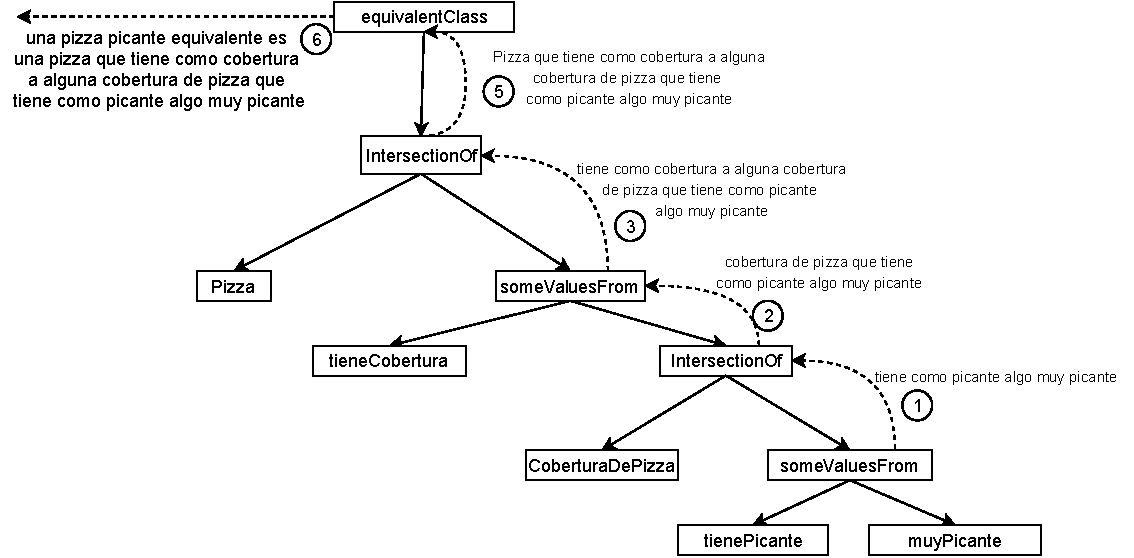
\includegraphics[width=\textwidth]{img/generacion_documento/verbalizacion_equivalentClass_spanish.pdf}
    \caption{Ejemplo gráfico de verbalización en lenguaje español.}
    \label{fig:ejemplo_verb_espaniol}
\end{figure}

\subsubsection{Axioma lenguaje inglés}
El ejemplo se tomó de la ontología Wine. El \textit{Axioma} se corresponde al constructor \emph{owl:equivalentClass} sobre la clase \emph{CheninBlanc}. El contenido del axioma es el siguiente: 

\begin{verbatim}
EquivalentClasses(
    :CheninBlanc
    ObjectIntersectionOf(
        :Wine
        ObjectHasValue(
            :madeFromGrape
            :CheninBlancGrape)
        ObjectMaxCardinality(
        1
        :madeFromGrape)
    )
)
\end{verbatim}
La verbalización se muestra en la Figura~\ref{fig:ejemplo_verb_ingles}.
Los pasos del proceso se encuentran enumerados desde el 1 al 4. Las gramáticas utilizadas son similares a las explicadas para lenguaje español, con la diferencia que los enlaces han sido traducidos a inglés.

Resulta conveniente explicar el paso N$^\circ$3 particularmente. El resultado de este paso es consecuencia de la intersección entre ``Wine'' y el resultado del paso 1 y 2. 
Como es una intersección de tres componentes, se procede a agrupar los componentes según su tipo, para luego unirlos a través de la conjunción ``y''. Dado que el operador \emph{hasValue} y \emph{minCardinality} retornan componentes de tipo SV, son agrupados juntos en una oración. Luego de agruparlos, se procede a realizar el proceso de agregación entre ambas, a través del cual se elimina el verbo ``made'' de la oración parcial construida en el paso 1. 

Por otro lado, la Clase Wine retorna un tipo T, por lo que queda aislado en una oración independiente. Estas agrupaciones resultan en el texto del paso Nº3.

La verbalización de este axioma da como resultado dos oraciones. Como ambas oraciones hacen referencia a la misma Clase, en el paso N$^\circ$4  se ejecuta el algoritmo para agregar Expresiones de Referencias, por lo que en la segunda oración se reemplaza el nombre de la Clase por la expresión \texttt{This}. En el paso N$^\circ$4 finaliza la verbalización del axioma y se retorna la oración completa.

\begin{figure}
    \centering
    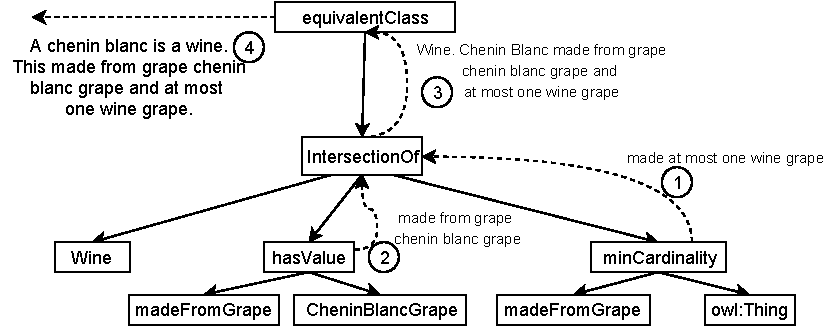
\includegraphics[width=\textwidth]{img/generacion_documento/verbalizacion_equivalentClass_english.pdf}
    \caption{Ejemplo gráfico de verbalización en lenguaje inglés.}
    \label{fig:ejemplo_verb_ingles}
\end{figure}

\subsection{Diagrama de clases}
En la Figura~\ref{fig:diagrama_clases_microplanificador} se puede ver el diagrama de clases asociado al módulo de Microplanificación. 
La clase \emph{Statement} es la encargada de realizar la verbalización de los constructores de Axiomas y las enumeraciones. Un objeto \emph{Statement} puede generar más de una oración, ya que cada \emph{Statement} trata un solo tópico y un solo tipo de constructor, pero pueden haber varios axiomas que utilicen el mismo tipo de constructor, por lo que todos esos axiomas estarán en la misma \emph{Statement}.

La clase \emph{StatementComponent} representa la oraciones parciales. Se encarga de componer oraciones parciales y generar una nueva oración parcial. En el caso de un constructor de \textit{Entidad}, se encarga de generar una oración parcial compuesta por el nombre de la entidad.

La clase \emph{Word} representa las palabras usadas durante la verbalización. Contiene la función gramatical de la palabra, y los algoritmos necesarios para convertir una palabra en plural, un número en palabra (1 a uno), cambiar el género de una palabra, retornar el artículo correspondiente a un sustantivo, entre otros.

Las subclases de \emph{OWLRestriction} tienen la capacidad de verbalizar los constructores de Expresiones de Clases y de generar las \emph{StatementComponent}.

\begin{figure}
    \centering
    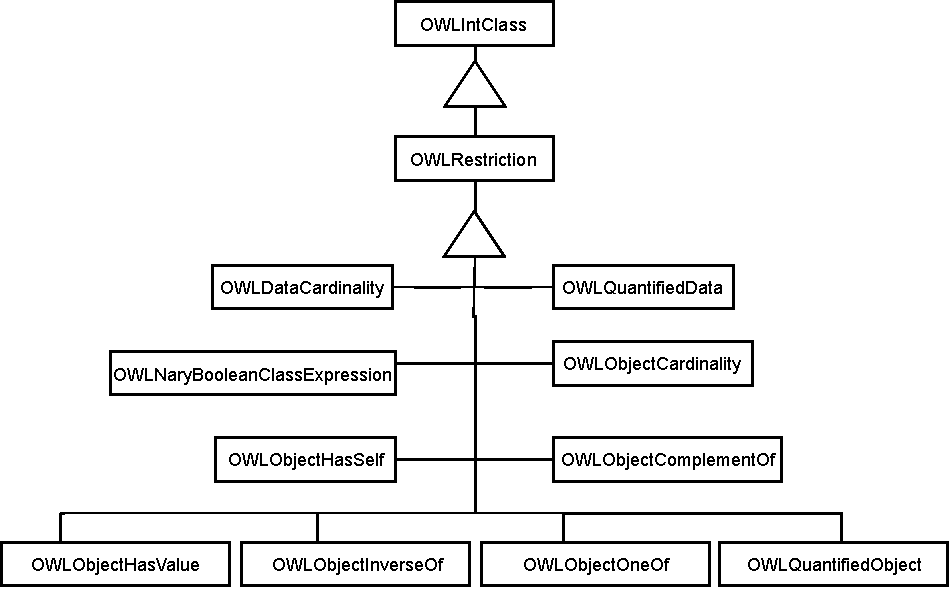
\includegraphics{img/generacion_documento/diagrama_clases_microplanificador.pdf}
    \caption{Diagrama de clases del Microplanificador.}
    \label{fig:diagrama_clases_microplanificador}
\end{figure}


\section{Implementación Microplanificador}
Para facilitar la implementación de los algoritmos de Agregación y Expresiones de Referencia, decidimos implementar el contenido de las oraciones con listas de palabras en lugar de cadenas de texto, facilitando su manipulación y recorrido. De esta manera, se creó la interfaz \emph{Word} con sus respectivas subclases \emph{WordEnglish} y \emph{WordSpanish}. 
La clase \emph{WordSpanish} utiliza la librería \emph{javaGramatica}\footnote{\url{https://www.proinf.net/permalink/gramatica_numero_genero_y_acentuacion}}, para implementar algunos métodos del idioma español, como pluralizar, cambio de género, número, etc. Para el idioma inglés estos métodos fueron implementados manualmente.

Cada vez que se crea una Word, debe especificarse su palabra y el tipo de función que cumple la palabra. Para identificar el tipo de una palabra, se utilizó el software \texttt{Stanford POS Tagger}\footnote{https://nlp.stanford.edu/software/tagger.html}, el cual permite etiquetar palabras de inglés, español y otros idiomas. Este software utiliza una nomenclatura específica para etiquetar las palabras (llamadas etiquetas \texttt{EAGLE}\footnote{\url{https://web.archive.org/web/20160325024315/http://nlp.lsi.upc.edu/freeling/doc/tagsets/tagset-es.html}} para el español, y para el inglés el \texttt{Penn Treebank}\footnote{\url{https://www.ling.upenn.edu/courses/Fall_2003/ling001/penn_treebank_pos.html}}), por lo que utilizamos esa nomenclatura y la implementamos a través de Variables de Clase creadas en la clase Word.

Los objetos \emph{Word} son creados por cada \emph{StatementComponent}. Una \emph{StatementComponent} se crea durante el proceso de verbalización de los constructores de Expresiones de Clase y de Entidades. Como los constructores del nivel más bajo son de Entidades, es en ellas donde se decide qué tipo de objeto se instancia según el idioma, es decir \emph{StatementComponentEnglish} o \emph{StatementComponentSpanish}. 

En el nivel de los constructores de Expresiones de Clase se encuentran las clases que heredan de la interfaz \emph{OWLRestriction}. Esta interfaz acopla los atributos que requieren los constructores, como los individuos, las clases, las propiedades y cardinalidades.

Las clases que implementan \emph{OWLRestriction} componen y generan las \emph{StatementComponent}. Como ejemplo, se muestra en la Anexo~\ref{sec:clase_OWLObjectComplementOf} la implementación de la clase \emph{OWLObjectComplementOf} con los métodos para implementar la verbalización del constructor en español.

Se puede ver que el método \emph{generateStatementSpanish()} recibe como párametro un objeto de clase \emph{TextCotext}. Esta clase tiene el tópico al que hace referencia la oración que se está componiendo y el lenguaje de la oración, para ser utilizados, por ejemplo, en la generación de Expresiones de Referencia.

Por último, la interfaz \emph{Statement} tiene los atributos necesarios para que sus implementaciones \emph{StatementEnglish} y \emph{StatementSpanish} puedan verbalizar los constructores de Axiomas y de unir todas las oraciones. 

Las \emph{Statement} utilizan la Agregación y las Expresiones de Referencia cuando generan varias oraciones. Estas tareas se implementaron en las clases \emph{StatementComponent} (teniendo en cuenta sus implementaciones) y \emph{OWLClass} respectivamente. En el Anexo~\ref{sec:met_exp_ref} se muestra el método usado para generar las Expresiones de referencia en la clase \emph{OWLClass}.


\section{Diseño del realizador}
%La arquitectura de este trabajo relegó la tarea de definir la estructura de las oraciones y llevar acabo su realización lingüística a la etapa de Microplanificación.
En esta etapa queda la tarea de definir la estructura final del documento. 
Alcanzaremos el Documento Final, a través del refinamiento del Documento Inicial creado en la Macroplanificación.

El Documento Inicial tiene una estructura en la que todos los tópicos tienen su propia sección, por lo que no existe más información que haga posible expandir la estructura. Por este motivo, nos enfocaremos en la idea de reducir la estructura del documento convirtiendo secciones en párrafos, para que se haga más compacto, tratando de mejorar la estética y el proceso de lectura, sin perjudicar la coherencia y la segmentación de la información.

Para llevar a cabo el refinamiento, se buscó medir la información a verbalizar, para saber cuándo es posible convertir una sección. Para esto se propuso como métrica principal a la cantidad de oraciones presentes en la descripción de un tópico.

\subsection{Criterio de reducción de Secciones}
Una sección agrupa uno o más párrafos o sub-secciones, por lo que en una sección puede existir más de un tópico, con la condición de que esos tópicos tengan una relación, ya sea de hermanos o de hijos. Estas relaciones se obtienen del Documento Inicial. 

Para decidir si un tópico es planificado como una Sección, se utilizan los siguientes criterios:
\begin{itemize}
    \item Debe poseer cinco o más oraciones.
    \item Debe poseer alguna Subsección con cinco o más oraciones.
    \item En cualquier otro caso será planificado como un Párrafo.
\end{itemize}

Si la cantidad de oraciones requeridas para ser considerada una sección tiende a cero, la planificación del documento será similar al Documento Inicial; mientras que si la cantidad de oraciones tiende a infinito, la planificación perderá niveles de jerarquía, y únicamente contemplará como secciones a los tópicos del primer nivel. Ninguno de los dos extremos es conveniente: o se pierde coherencia, o se obtiene un texto con demasiados niveles de secciones, que resulta antinatural. Sin embargo, un documento en el que predominan las sub-secciones (aunque tengan poca información), ayuda a los humanos a reconocer y establecer relaciones entre los tópicos, siendo el objetivo principal no desaprovechar la semántica del dominio modelado, y teniendo como intención principal que el lector comprenda el dominio modelado en la ontología.

\section{Implementación del Realizador}
El Realizador está embebido dentro de la \textit{clase }\textit{Section}, en forma de métodos que implementan los criterios vistos para la definición del documento. En el Anexo~\ref{sec:clase_section} se presenta un pseudocódigo de la\textit{ clase }\textit{Section}.

\section{Casos de estudio}
En el Capítulo~\ref{cap:organizacion} de Organización de información analizamos cómo quedan organizados los tópicos de las ontologías Pizza y Wine, por lo que continuaremos con estas ontologías de ejemplo, analizando la realización del texto generado. Para identificar el formato del texto, a las secciones se le incluye el número de sección a la izquierda del título de la sección, y cada párrafo comienza con sangría.

Debido a que existen una gran cantidad de  parámetros a tener en cuenta en el análisis de un texto, consideraremos aquellos que estén directamente relacionados con el objetivo propuesto: 

\begin{itemize}
    \item Con relación a la estructura jerárquica del texto, analizaremos la coherencia global y si los temas son representativos de la ontología.
    \item Respecto a la sintaxis, veremos si las oraciones son claras, cumplen con la sintaxis del idioma, son coherentes a nivel local, y si transmiten el significado del axioma verbalizado. 
    \item En cuanto a la realización del texto, analizaremos la estética (aunque de manera subjetiva), viendo si la segmentación en secciones y párrafos es agradable.
\end{itemize}


\subsection{Generación documento ontología Pizza}
Por causa de que el texto completo resulta muy extenso, solo pondremos los fragmentos más significativos del Documento Final. En la Figura~\ref{fig:doc_final_pizza} se presentan los fragmentos a analizar. Para visualizar la estructura total del documento, se imprimió el índice de las secciones, el cual se muestra en la Figura~\ref{fig:indice_secciones_pizza}. 

Los tópicos reconocidos representan adecuadamente el tema del texto. Se puede apreciar que la estructura del documento comparte algunas similitudes con el Documento Inicial, manteniendo la coherencia global, pero disminuyó la cantidad de secciones, ya que muchas de ellas se convirtieron en párrafos. Aún así, prevalecen títulos de secciones que agregan información semántica aunque no aporten información en forma de texto, tales como Ingredientes, Coberturas y Bases.

La sintaxis es aceptable y las oraciones pueden comprenderse, aunque pueden mejorarse para disminuir la redundancia. Los axiomas no son muy complejos, aunque verbalizó bien axiomas de hasta cuatro niveles de jerarquía, como el de la Figura~\ref{fig:ejemplo_verb_espaniol}. Las oraciones resultan coherentes, el salto entre oraciones es fluido teniendo en cuenta que no intercalan tópicos, y el contenido del texto anticipa bien la aparición de párrafos y subsecciones.

La estructura de las oraciones es repetitiva, no era el objetivo de este trabajo realizar un texto variado, por lo que ante la misma información para verbalizar se obtiene la misma estructura.

En cuanto a la cuestión estética, el texto resulta aceptable, no posee muchas secciones anidadas por lo que visualmente no sobrecarga la lectura.

\begin{figure}
\centering
\fbox{
\begin{minipage}{14cm}
\setlength{\parindent}{1em}
\large{
\noindent 1 Pizza
}

\small{
Una pizza es una comida. Una pizza tiene base de pizza y tiene cobertura de pizza. Esta tiene como base a alguna base de pizza. Existen las siguientes clases de pizzas: pizza con carne, picante, no vegetariana, con nombre, \dots, con queso y vegetariana. Una pizza es disjunta de base de pizza, cobertura de pizza y helado.

Pizza con carne: una pizza con carne es una pizza que tiene como cobertura a alguna cobertura de carne. 

Pizza vegetariana equivalente1: una pizza vegetariana equivalente1 es una pizza que tiene como cobertura exclusivamente a cobertura vegetariana.

Pizza picante equivalente: una pizza picante equivalente es una pizza que tiene como cobertura a alguna cobertura de pizza que tiene como picante algo muy picante. 

Pizza real italiana: una pizza real italiana es una pizza que tiene pais de origen italy. Esta tiene como base exclusivamente a base delgada y crujiente.

\par \dots Otras pizzas realizadas como párrafos.
}

\large{
\noindent 1.1 Pizza con nombre
}

\small{
Una pizza con nombre es una pizza. Existen las siguientes clases de pizzas con nombre: margherita, frutti di mare, \dots, veneziana y napoletana.

Margherita: una margherita es una pizza con nombre. Esta tiene como cobertura a alguna cobertura de mozzarella y tomate. También, margherita tiene exclusivamente las siguientes coberturas: cobertura de mozzarella o de tomate. una margherita es disjunta de american, american hot, \dots, soho y veneziana.

\dots Otras pizzas con nombre realizadas como párrafos.
}

\large{
\noindent 1.2 Ingredientes
	
\noindent 1.2.1 Coberturas
	
\noindent 1.2.1.1 Cobertura de pizza
}

\small{
Una cobertura de pizza es una comida. Una cobertura de pizza es cobertura de una pizza. Existen las siguientes clases de coberturas de pizza: \dots
}

\large{
\noindent 1.2.2 Bases
}

\large{
\noindent 1.2.2.1 Base de pizza
}

\small{
Una base de pizza es una comida. Una base de pizza es base de una pizza. Existen las siguientes clases de bases de pizza: base gruesa y delgada y crujiente.
}
\end{minipage}
}
\caption{Fragmentos del Documento Final generado a partir de la ontología Pizza.}
\label{fig:doc_final_pizza}
\end{figure}

\begin{figure}
\begin{multicols}{2}
\small{
\begin{figure}[H]
\dirtree{%
.1 Pizza.
.2 Pizza con nombre.
.2 Ingredientes.
.3 Coberturas.
.4 Cobertura de pizza.
.5 Cobertura de verduras.
.6 Cobertura de pimiento.
.6 Cobertura de tomate.
.5 Cobertura de hierbas.
.5 Cobertura de carne.
.5 Cobertura de queso.
.5 Cobertura de pescado.
.3 Bases.
.4 Base de pizza.
.5 Base gruesa.
.5 Base delgada y crujiente.
}
\end{figure}

\begin{figure}[H]
\dirtree{%
.1 Otras secciones.
.2 Domain concept.
.3 Comida.
.2 Value partition.
.3 Picante.
}
\end{figure}
}
\end{multicols}
\caption{Índice de secciones del Documento Final generado para la ontología Pizza.}
\label{fig:indice_secciones_pizza}
\end{figure}


\subsection{Generación documento ontología Wine}
Al igual que el caso de estudio anterior, solo incluiremos algunos fragmentos del documento generado, los cuales se pueden ver en la Figura~\ref{fig:doc_final_wine}.

En la Figura~\ref{fig:indice_secciones_wine} se visualiza el índice del documento. El resultado es similar al obtenido en la verbalización de la ontología Pizza, comparando la Figura~\ref{fig:indice_secciones_wine} con la Figura~\ref{fig:caso_estudio_wine}, se observa que la estructura resulta mucho más compacta.

Analizando la coherencia global y el sentido del texto, la estructuración resultó razonable, enfocada en los vinos y las propiedades de los vinos.

La implementación de la sintaxis es sustancialmente equivalente a la del español, por lo que puede presentar las mismas características y capacidades, como redundancia, repetitividad y claridad. 

El resultado de la realización final también resulta satisfactorio. Si bien presenta hasta cinco niveles de anidamiento (a partir de \emph{Consumable thing}), la información que se transmite es necesaria para mantener la coherencia global y establecer las relaciones pertinentes entre los tópicos.

\begin{figure}
\centering
\fbox{
\begin{minipage}{14cm}
\setlength{\parindent}{1em}
\large{
\noindent 1 Wine
}

\small{
A wine is a potable liquid. A wine has wine sugar as sugar, has wine flavor as flavor, has wine body as body, has wine color as color, has wine descriptor and made from grape a wine grape. This located in some region. Also, wine has only winery maker. Also, wine has exactly one maker, made at least one wine grape, wine body, wine color, wine flavor and wine sugar. There are the following kinds of wines: italian wine, \dots, late harvest and alsatian wine. 

Full bodied wine: a full bodied wine is a wine that has full body.

Burgundy: a burgundy is a wine that located in bourgogne region. This has dry sugar. There are the following kinds of burgundies: white burgundy and red burgundy. 

\dots Otros vinos realizados como párrafos.
}

\large{
\noindent 1.1 Italian wine
}

\small{
A italian wine is a wine that located in italian region. chianti is the only kind of wine. 

Chianti: a chianti is a italian wine. This has only light or medium body. Also, chianti has red color, moderate flavor and dry sugar. located in chianti region. made from grape sangiovese grape. chianti classico is a type of chianti. 

Chianti classico: a chianti classico has mc guinnesso maker and medium body.
}

\large{
\noindent 1.2 ... 1.7
}

\large{
\noindent 1.8 Red wine
}

\small{
A red wine is a wine that has red color. There are the following kinds of wines: dry red wine, red burgundy, port and red bordeaux. 

Port: a port is a red wine. This has full body, strong flavor and sweet sugar. located in portugal region. taylor port is a type of port. 
Taylor port: a taylor port has taylor maker. 
}


\large{
\noindent 1.8.1 Red burgundy
}

\small{
A red burgundy is a burgundy and red wine. This made from grape pinot noir grape. Also, red burgundy made at most one wine grape. cotes d or is the only kind of burgundy. 
Cotes d or: a cotes d is a red burgundy that located in cotes d or region. This has moderate flavor. clos de vougeot cotes d or is a type of cotes d or. 
Clos de vougeot cotes d or:	a has clos de vougeot maker. 
}

\small{\dots Otros vinos realizados como secciones}

\large{
\noindent 1.14 Wines descriptor
}

\small{
Wine sugar:	a wine sugar is a wine taste. a wine sugar is a sweet, off dry or dry. there are the wines sugar: dry, off dry and sweet. 

Wine color: a wine color is a wine descriptor. a wine color is a rose, red or white. there are the wines color: white, red and rose. 

Wine flavor: a wine flavor is a wine taste. a wine flavor is a moderate, delicate or strong. there are the wines flavor: moderate, strong and delicate. 

Wine body: a wine body is a wine taste. a wine body is a light, medium or full. there are the wines body: medium, full and light. 
}

\large{
\noindent Otras secciones menos importantes
}

\large{
\noindent 2 Region
}

\small{
A region adjacent region. There are the regions: arroyo grande region, california region, ....

Arroyo grande region: an arroyo grande region located in california region. 

....
}

\large{
\noindent 3 Vintage year
}

\small{
A vintage year has year value. year1998 is a type of year. 
Year1998: a year1998 has year value. a year1998 has year value. 
}

\small{
\dots Otras secciones.
}

\end{minipage}
}
\caption{Fragmentos del Documento Final generado a partir de la ontología Wine.}
\label{fig:doc_final_wine}
\end{figure}


\begin{figure}
\begin{multicols}{2}
{\small
\begin{figure}[H]
\dirtree{%
.1 Wine.
.2 Italian wine.
.2 Loire.
.2 Table wine.
.2 Pinot noir.
.2 Dessert wine.
.3 Sweet riesling.
.2 Bordeaux.
.3 Medoc.
.2 Riesling.
.2 Red wine.
.3 Red burgundy.
.2 Cabernet sauvignon.
.2 Semillon or sauvignon blanc.
.3 Sauvignon blanc.
.2 White wine.
.3 White burgundy.
.2 Zinfandel.
.2 Chardonnay.
.2 Wines descriptor.
.3 Wine sugar.
.3 Wine color.
.3 Wine flavor.
.3 Wine body.
}
\end{figure}}  

\begin{figure}[H]
\dirtree{%
.1 Otras secciones.
.1 Region.
.1 Vintage year.
.1 Wine descriptor.
.1 Non consumable thing.
.1 Vintage.
.1 Fruit.
.1 Winery.
.1 Consumable thing.
.2 Meal course.
.3 Foods.
.4 Edible thing.
.5 Seafood.
.5 Pasta.
}
\end{figure}

\end{multicols}
\caption{Índice de secciones del Documento Final generado para la ontología Wine.}
\label{fig:indice_secciones_wine}
\end{figure}


Dado que en lenguaje inglés hay ejemplos de verbalizaciones de otras investigaciones, a continuación se presenta una comparación de la verbalización de la clase \emph{Beaujolais} de la ontología \emph{Wine}, entre el trabajo~\cite{hewlett2005effective} y el nuestro:

En~\cite{hewlett2005effective} proponen listar sus características de la siguiente manera: 
``A Beaujolais is a Wine that:
\begin{itemize}
    \item is made from at most 1 grape, which is Gamay Grape
    \item has Delicate flavor
    \item has Dry sugar 
    \item has Red color
    \item has Light body ''
\end{itemize}

En nuestro caso, la oración resultante es la siguiente:
``Beaujolais has light body, red color, delicate flavor and dry sugar. Made from grape gamay grape.''

Existe clara diferencia, no solo en el criterio de presentación lista frente a prosa, sino también en el hecho de elegir cuánta elipsis emplear (en nuestro caso, además de omitir Beaujolais, también omitimos el verbo ``has'' para evitar redundancia), y de separar en diferentes oraciones las características asociadas al ``has'' y las asociadas al ``made from''. Decidir qué representación usar depende de muchos factores, por ejemplo, la versión en prosa no resulta muy compleja, pues la omisión del ``has'' solo ocurre en tres características, por lo que no recae tanta carga sobre el lector. Quizá en descripciones más largas sea conveniente un formato en lista, pero también hay que tener en cuenta cómo impactaría visualmente representar todas las clases de una gran ontología de esta forma. De acuerdo con~\cite{hewlett2005effective}, pueden existir métodos de generación más complejos que mejoren la calidad del texto de salida.

Otra herramienta que se pudo probar con la ontología \emph{Wine} fue Attempto Tools~\cite{attempto}, la cual retornó la siguiente salida para la clase Beaujolais:

``
Every Beaujolais hasBody Light.

Every Beaujolais hasColor Red.

Every Beaujolais hasFlavor Delicate.

Every Beaujolais hasSugar Dry.

Every Beaujolais madeFromGrape GamayGrape.

Every Beaujolais madeFromGrape at most 1 thing.
''

En comparación con las salidas en formato lista y prosa, podemos apreciar que esta salida es la que menos trabaja sobre las oraciones, repitiendo información y dejando la nomenclatura camelCase sin procesar.

\section{Conclusiones}
Hemos presentado un sistema que genera un texto en lenguaje natural a partir de los axiomas de una ontología. La estructura del documento de texto depende de la organización realizada en el Macroplaning, y de los criterios tomados en el Realizador, conservando la coherencia global recibida del Organizador de Información. 

Tomando como referencia lo postulado por la Teoría de Centrado, se pudo proveer a los párrafos de coherencia local. Para cada clase se reunió la mayor cantidad de información disponible, agrupándola a través de los constructores de Axiomas.

La separación en constructores de Expresiones de Clases y constructores de Axiomas, dio lugar a las oraciones parciales y a un sistema de tipos. Si bien este sistema no se corresponde fielmente a las categorías de constituyentes sintácticos\footnote{Un constituyente sintáctico es una palabra, o secuencia de palabras, que funciona en conjunto como una unidad dentro de la estructura jerárquica de una oración} de alguna gramática conocida (como la gramática tradicional o la gramática generativa\footnote{La gramática tradicional y la generativa se enfocan en el estudio de la gramática del lenguaje. La gramática generativa es más moderna y estudia la sintaxis del lenguaje a través de definiciones formales.} ), permitió minimizar la cantidad de combinaciones que había que diseñar en las gramáticas.

Las sentencias fueron debidamente procesadas para aplicar algunas técnicas de Procesamiento de Lenguaje Natural, como expresiones de referencia, agregación de sentencias, inflexión de número y determinación de pronombres basados en el género (en el caso del lenguaje español). 

El resultado en los casos de prueba fue satisfactorio, la sintaxis generó oraciones interpretables.

Como mostramos en las comparaciones con resultados de otros trabajos, es posible tomar diferentes criterios para mostrar la misma información, y desarrollar técnicas o gramáticas más sofisticadas para mejorar la fluidez del texto.